\documentclass[a5paper,11pt,landscape]{report}
\usepackage[utf8]{inputenc}
\usepackage[a5paper,includemp,
      scale={0.9,0.85},
      includeheadfoot,
      bindingoffset=0cm]{geometry}
% This is an annotated latex definition file.
% You can give it any name as long as its inputted somewhere
% in your code.
% You may even put it in a directory other then the current
% as long as that directory is in the TEXINPUTS path.
% Comments start with a % as you a seeing right now. Otherwise look
% to the left.
% font of the times family
%\usepackage{palatino}
\usepackage{lmodern}
% make linenumbering possible for reviewing
\usepackage[pagewise,mathlines,displaymath]{lineno}
% use the pdftex graphics extensions
\usepackage{graphicx}
\usepackage{wrapfig}
% to make the headers and footers look nice
\usepackage{xcolor,fancyhdr}
% allow drawing with tikz
\usepackage{tikz}
% allow compact lists etc.
\usepackage{enumitem}
% make the header (and footer) span the whole printable area
\addtolength\headwidth\marginparwidth
\addtolength\headwidth\marginparsep
\pagestyle{fancy}
\usepackage[all]{svn-multi}
\svnRegisterAuthor{879417}{Pieter van den Hombergh}

% \usepackage{svn}
\newcommand\TheFile{mydefs.tex}
\newcommand\Code[1]{\textbf{\texttt{#1}\ }}
%%
% to get version information in files, include the following lines in
% each document 
% and renewcommand\TheFile to something like \renewcommand\TheFile{main.text}
%\renewcommand\footrulewidth{1pt}
% put revision control info in the footer
% the vspace compensates for the space taken up by the logo on the right hand.
% I like a fontys color in my header
\definecolor{purple}{rgb}{0.21,0,0.21} % a darkish purple
\renewcommand\headrule{%
  {\color{purple}%
    \hrule height 2pt width \headwidth
    \vspace{1pt}%
    \hrule height 1pt width \headwidth
    \vspace{-4pt}%
  }%
}%
\renewcommand\footrule{
  {\color{purple}%
    \hrule height 1pt width \headwidth
    \vspace{1pt}%
    \hrule height 2pt width \headwidth
    \vspace{2pt}%
  }%
}
% do not indent pars, increase parskip
\setlength\parindent{0pt}
\setlength\parskip{0.5em}
% my own itemize: a bit less spacy then the default
\newenvironment{Itemize} {
  \begin{itemize}{}%
    \setlength\topsep{0ex}%
    \setlength\parskip{0ex}%
    \setlength\partopsep{0em}%
    \setlength\parsep{0em}%
    \setlength\itemsep{0em}%
    }%
  {\end{itemize}}
% make the head a bit heigher
\setlength\headheight{16pt}
\setlength\footskip{60pt}
%%
% This macro '\define' puts the argument in em 
% and in boldface in the margin.
\newcommand{\define}[1]{% 1 argument
  \mbox{}{\textit{#1}}% italics or em
  \marginpar{\raggedright% no adjust
    \bfseries\hspace{0pt}#1}% bold
} % end of macro

%%
% At start of pages, define sometimes puts the material in the wrong margin
% in that case use this fix.
\newcommand{\fixdefine}[1]{\mbox{}{\textit{#1}}%
  \reversemarginpar\marginpar{\bfseries\hspace{0pt}#1}\normalmarginpar}
% to display source code like things
\usepackage{listings}
\lstset{numbers=right} % to get out of the way with document line numbers
% to be able to 'on this page' and the like
\usepackage{varioref}
% to put a nice quote with the chapter
\usepackage[avantgarde]{quotchap}
\renewcommand\chapterheadstartvskip{\vspace*{-5\baselineskip}}
%select Helvetica for title and quote
\usepackage{helvet}
\renewcommand\sectfont{\sffamily\bfseries}

%% example
%\begin{savequote}[10cm]
% \sffamily
%some text
%\end{savequote}
% needed for inclusion of gnumeric table
\def\inputGnumericTable{}
%% 
\usepackage{array}    
\usepackage{longtable}
\usepackage{calc}     
\usepackage{multirow} 
\usepackage{hhline}   
\usepackage{ifthen}   
%%
% Fancy headers are used
% To make the footer appear on chapter pages too,
% we redefine the fancypagestyle plain
\fancypagestyle{plain}{%
  \fancyhf{} % clear all  
  \fancyfoot[RO,LE]{\vspace{-1.2cm}%
  File: \svnkw{Filename}\\%
  Author: \svnFullAuthor*{\svnfileauthor}\\%
  Revision: \svnrev, \svnyear-\svnmonth-\svnday\ \svnhour:\svnminute\\
}
  \fancyfoot[RE,LO]{
\includegraphics[width=2cm]{figures/fon000_00c.pdf}}
  \fancyfoot[C]{\bfseries\thepage}
  \renewcommand\headrule{}%
}% end of redef fancypagestyl plain
% Define my own fancy headers and footers  
\fancyhead{}
\fancyhead[RO]{\rightmark} % display section name
\fancyhead[LE]{\rightmark}
\fancyfoot[RO,LE]{\vspace{-1.2cm}%
  File: \svnkw{Filename}\\%
  Author: \svnFullAuthor*{\svnfileauthor}\\%
  Revision: \svnrev, \svnyear-\svnmonth-\svnday\ \svnhour:\svnminute\\
}
% logo in footer
\fancyfoot[RE,LO]{
\includegraphics[width=2cm]{figures/fon000_00c.pdf}}
\pagestyle{fancy}
\usepackage{fontyscoverpage}
%%
% For a watermark on each page:
\usepackage{eso-pic} % needed package
% Draw a DRAFT through the text.
% for other text renewcommand the next command
\newcommand\watermarktext{Draft}
% You could make this depend on the status of the files.
\makeatletter
  \AddToShipoutPicture{%
    \setlength{\@tempdimb}{.5\paperwidth}%
    \setlength{\@tempdimc}{.5\paperheight}%
    \setlength{\unitlength}{1pt}%
    \put(\strip@pt\@tempdimb,\strip@pt\@tempdimc){%
      \makebox(0,0){\rotatebox{55}{% for longer texts you might want to increase this angle
          \textcolor[gray]{0.85}{% the higher the number, the lighter the text
            \fontsize{8cm}{8cm}% Fit this font to the text
            \sffamily
            \selectfont{\watermarktext}}}}
    }
}
\makeatother
\lstdefinelanguage{BibTeX}
  {keywords={%
      @article,@book,@collectedbook,@conference,@electronic,@ieeetranbstctl,%
      @inbook,@incollectedbook,@incollection,@injournal,@inproceedings,%
      @manual,@mastersthesis,@misc,@patent,@periodical,@phdthesis,@preamble,%
      @proceedings,@standard,@string,@techreport,@unpublished%
      },
   comment=[l][\itshape]{@comment},
   sensitive=false,
  }

% thenext comments are inserted by Emacs, that uses it 
% to process this latex file
%%% Local Variables: 
%%% mode: latex
%%% TeX-master: t
%%% End: 

\svnidlong{$HeadURL: https://www.fontysvenlo.org/svnp/879417/latexcolloquium/trunk/latexsample/screen.tex $}%
{$LastChangedDate: 2013-09-08 12:54:29 +0200 (Sun, 08 Sep 2013) $}%
{$LastChangedRevision: 31 $}%
{$LastChangedBy: 879417 $}
\svnid{$Id: screen.tex 31 2013-09-08 10:54:29Z 879417 $}
\renewcommand\TheFile{screen.tex}

%
% hyperef last, after all other packages
% this allows you to add hyperlinks in the document.
% It makes viewing it with e.g. Adobe acrobat very nice.

\usepackage[pdftex,colorlinks=false,
    pdfstartview=FitV,
    linkcolor=blue,
    citecolor=blue,
    urlcolor=blue,
    ]{hyperref}
\pdfinfo{
  /Title      (Sample latex document)
  /Author     (Pieter van den Hombergh 879417)
  /Keywords   (latex documentation graphics math listings)
}

%%
% Fancy headers are used
% To make the footer appear on chapter pages too,
% we redefine the fancypagestyle plain
\fancypagestyle{plain}{%
  \fancyhf{} % clear all  
  \fancyfoot[RO,LE]{%
  Revision: \svnrev, \svndate\\
}
  \fancyfoot[RE,LO]{
\includegraphics[width=1cm]{figures/fon000_00c.pdf}}
  \fancyfoot[C]{\bfseries\thepage}
  \renewcommand\headrule{}%
}% end of redef fancypagestyl plain
% Define my own fancy headers and footers  

\setlength{\unitlength}{1mm}
\fancyhead{}
\fancyhead[LO,LE]{\leftmark} % display section name
\fancyhead[RO,RE]{\rightmark}
\fancyfoot[RO,LE]{%
  Revision: \svnrev, \svndate\\
}
% logo in footer
\fancyfoot[RE,LO]{
\includegraphics[width=1cm]{figures/fon000_00c.pdf}}
\pagestyle{fancy}
\renewcommand\footrule{}
% every document needs a start and an end
\author{Pieter van den Hombergh\\879417}
\title{Sample \LaTeX\ document}
%\includeonly{intro}
\begin{document}
% lets have a default title page
\svnidlong{$HeadURL: https://www.fontysvenlo.org/svnp/879417/latexcolloquium/trunk/latexsample/screenfrontpage.tex $}%
{$LastChangedDate: 2013-09-08 12:54:29 +0200 (Sun, 08 Sep 2013) $}%
{$LastChangedRevision: 31 $}%
{$LastChangedBy: 879417 $}
\svnid{$Id: screenfrontpage.tex 31 2013-09-08 10:54:29Z 879417 $}
\renewcommand\TheFile{screenfrontpage.tex}

%%%%%%%%%%%%%%%%%%%%%%%%%%%%%%%%%%%%%%%%%%%%%%%%%%%%%%%%%%%%%%%%%%%%%%%%%%
%   This is frontpage.tex file needed for the dmathesis.cls file.  You   %
%  have to  put this file in the same directory with your thesis files.  %
%                Written by M. Imran 2001/06/18                          % 
%                 No Copyright for this file                             % 
%                 Save your time and enjoy it                            % 
%                                                                        % 
%%%%%%%%%%%%%%%%%%%%%%%%%%%%%%%%%%%%%%%%%%%%%%%%%%%%%%%%%%%%%%%%%%%%%%%%%%%
%%%%%%%%%%%%%%%%%%%%%%%%%%%%%%%%%%%%%%%%%%%%%%%%%%%%%%%%%%%%%%%%%%%%%%%%%%%
%%%%%%%%%%%%%%%%           The title page           %%%%%%%%%%%%%%%%%%%%%%%  
%%%%%%%%%%%%%%%%%%%%%%%%%%%%%%%%%%%%%%%%%%%%%%%%%%%%%%%%%%%%%%%%%%%%%%%%%%%
\pagenumbering{roman}

\newpage
{
\setlength{\unitlength}{1mm}
\begin{picture}(0,0)(15,122)
\put(0,0){\fbox{
\includegraphics[width=215mm]{figures/fontys-page-screen}}}
\put(60,140){\color{white}\Huge \bf \sf A \LaTeX{} screen reading sample}
\put(100,130){\color{white}\sf\Large{Fontys Venlo Software Engineering series}}
%% \put(5,2){\begin{minipage}[b]{\textwidth}
%%     \parindent=0in\raggedright
%%     {\large \sffamily\color{gray}
%%       Fontys Hogeschool voor Techniek en Bedrijfsmanagement\\
%%       Hogere Informatica/ Software Engineering\\
%%       Hulsterweg 2-6 Venlo\\
%%       The Netherlands\\
%%     }
%%   \end{minipage}}
\end{picture}
}
\thispagestyle{empty}
\begin{center}
  %\vspace*{4cm}
%\begin{minipage}[b]{\textwidth}
%% \parindent=0in\raggedleft
%% {\Huge \bf \sf \makeatletter\@title\makeatother}

%% \noindent{\Large\sffamily A sample file to showcase \LaTeX}
%% %\vspace*{2cm}

%% \noindent{\LARGE\bf\makeatletter\@author\makeatletter}

%% %\vspace*{20mm}
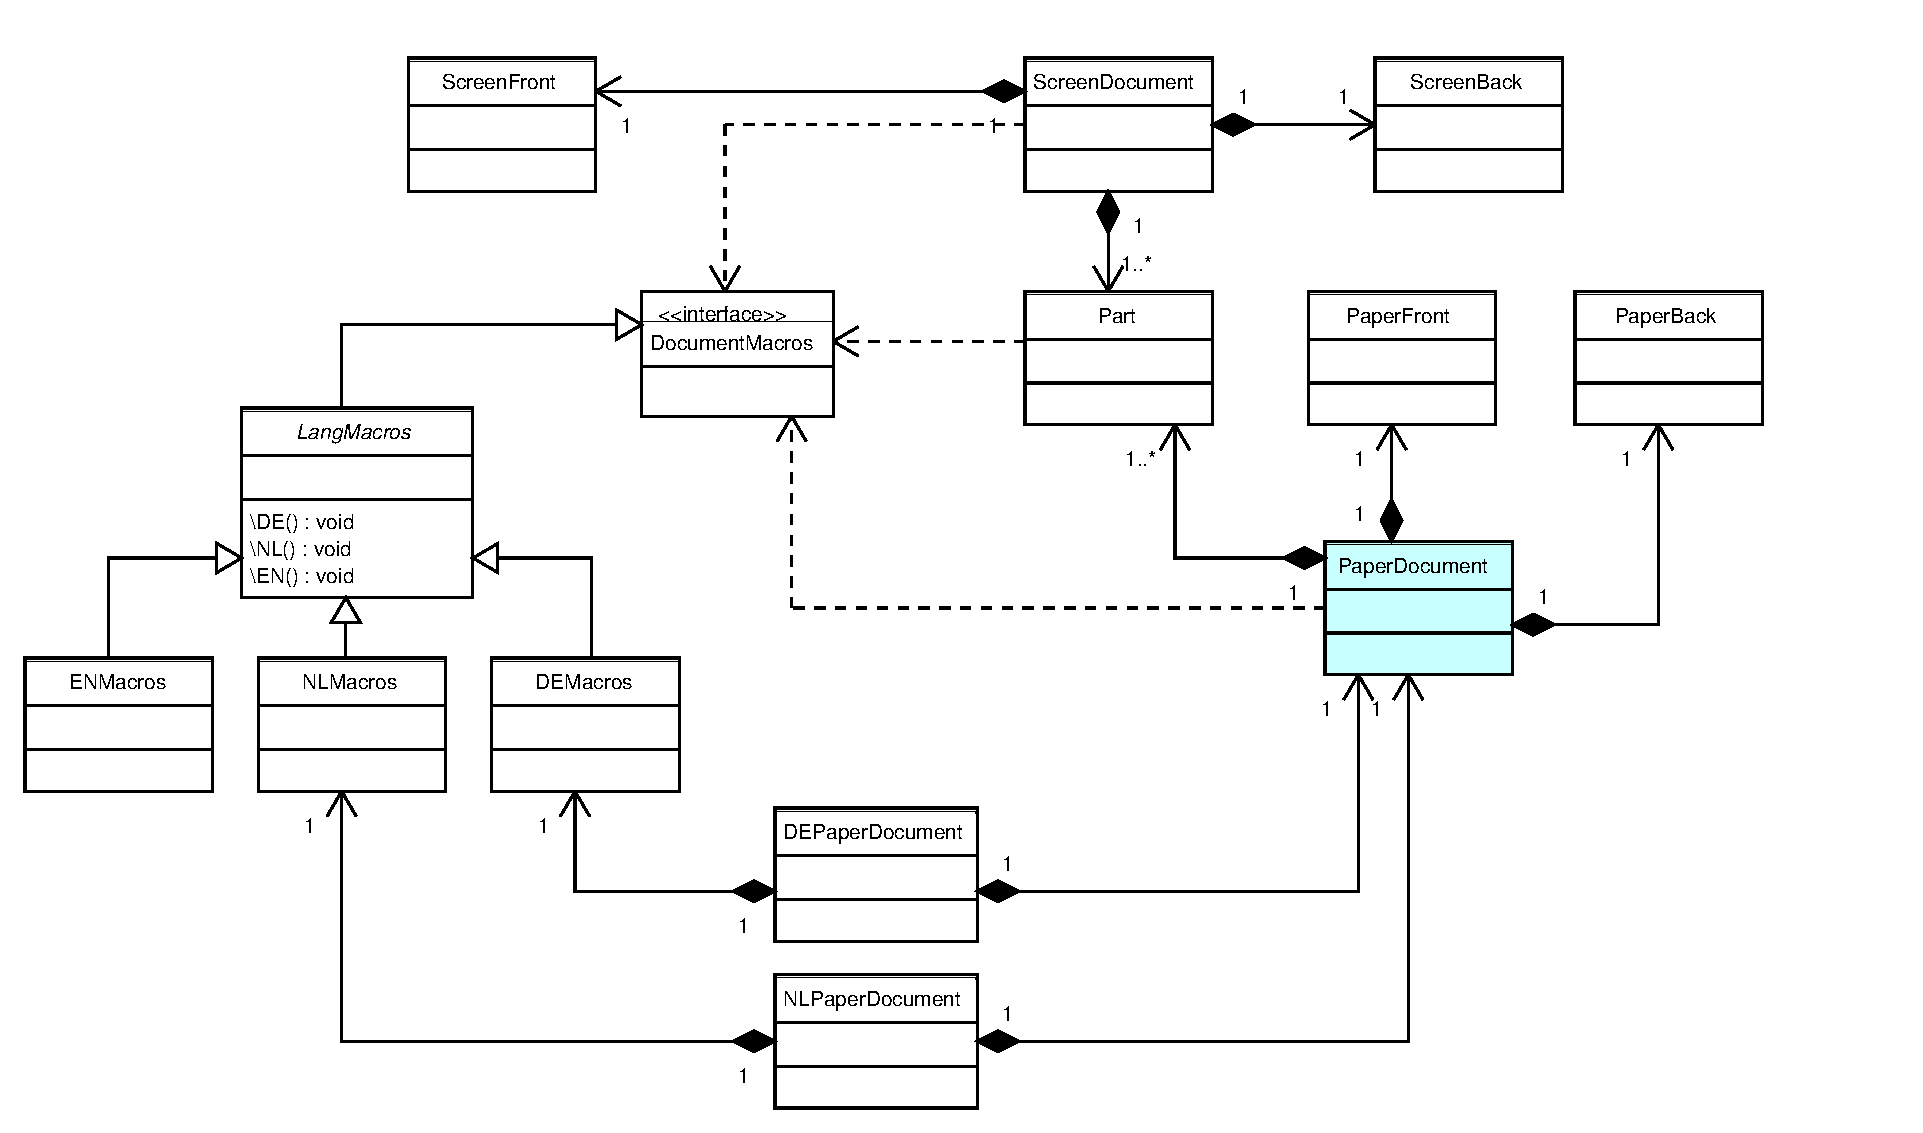
\includegraphics[width=.8\textwidth]{figures/latexfiles}
%\end{minipage}
\end{center}
%empty backside of frontpage
\pagestyle{empty}
\cleardoublepage
\setcounter{page}{1}
%%% Local Variables: 
%%% mode: latex
%%% TeX-master: "main"
%%% End: 

% I want a TOC
\pagestyle{fancy}
\tableofcontents
\newpage
\listoffigures
% The first chapter is in file intro
% this is a comment
% the next few lines include the other chapters.
% If the chapter files are not present they will simply not be found
% at most a warning is produced.
\renewcommand\watermarktext{}%{Fontys}
\cleardoublepage
\linenumbers
\svnidlong{$HeadURL: https://www.fontysvenlo.org/svnp/879417/latexcolloquium/trunk/latexsample/intro.tex $}%
{$LastChangedDate: 2014-11-16 16:03:56 +0100 (zo, 16 nov 2014) $}%
{$LastChangedRevision: 62 $}%
{$LastChangedBy: 879417 $}
\svnid{$Id: intro.tex 62 2014-11-16 15:03:56Z 879417 $}

\renewcommand\TheFile{intro.tex}

% quote text
\begin{savequote}[8cm]
  \sffamily
  Introducing oneself properly is always hard.
  \qauthor{Anonymous}
\end{savequote}
\chapter{Introduction}
\pagenumbering{arabic}
\setcounter{page}{1}
One of the standards for documentation in open source and hence in
Linux land is \LaTeX, a text processing package. \LaTeX\ is available
for free and available with all Linux distributions and installed in
the Lab.

\TeX\ is the machinery of \LaTeX\ and was defined in the \TeX\ book
\citep{texbook} and implemented by
Prof. Donald Knuth. \LaTeX\ is a (nowadays HUGE) set of macros built
on top of that. \LaTeX\ in its initial form is described by Leslie
Lamport in \citep{latexbook}. If you like your book thick, try the
\LaTeX\ companion \citep{latexcompanion}.

The web is also a very good source of \LaTeX\ documentation. A good
starting point is \url{http://en.wikibooks.org/wiki/LaTeX}, useful for
beginners and pros alike.

This is a simple multi part document. It's purpose is to show how easy it is
to create a multi part document, one that, for instance, can be worked on 
simultaneously by several authors. Note that most of the settings for
this document are set in the file \texttt{mydefs.tex}. 
Look in that file too.

This document consists of the following files
\begin{enumerate}[noitemsep,topsep=0pt,parsep=0pt,partopsep=0pt]
\item \texttt{main.tex}
\item \texttt{motivation.tex}
\item \texttt{graphics.tex}
\item \texttt{codelisting.tex}
\item \texttt{poser.tex}
\item \texttt{hello.c}
\item \texttt{Makefile} and
\item \texttt{mydefs.tex}
\item \texttt{servlet3.png}, the pie chart
\item \texttt{Diagram1.pdf}, the UML diagram
\end{enumerate} 

You are kindly advised to keep your lab logs in simple text
files. These can be turned into latex files easily,
which can be used to produce a nice looking report.
\clearpage 
\section{Some hints to start with}
Sometimes things do not work out the way you think.
\LaTeX\ interpretes some character codes in it's own way.
Things like dollar signs or even underscore are special.
\LaTeX\ source are littered with accolades or \textit{curly braces} if that's
the way you call them. They are special too. So here is some advice: 

Do not use \define{funny file names}. That is: stick to ASCII filenames without spaces or even underscores. 
These will bring only you into trouble. If you want to keep things portable, 
don't use camel case (like in JavaClassNames) either, because
some OS-es do not distinguish between upper and lower case. You may of
course brake this rule if the files are program things like
Java source files.

\subsection{Hints for informatics (use version control)}
In software projects, versioning is important. \LaTeX\ and \textsc{SubVersion}
work nicely together here.
By using the \LaTeX\ package \texttt{svn-multi} you can have svn+
latex insert meta information about your files in the produced output,
for instance in the page footers, as in this document.

If you add the codes below at the top of each .tex file, these
codes will be expanded/updated by svn \textit{on checkin}. 
% do not expand keywords on  the example file
\lstinputlisting{svnkeywords.head}
You must also tell
subversion to expand these keywords for those files with for each file
the command:\\
{\lstset{language=sh,numbers=none,morekeywords={svn,propset,keywords,filename},keywordstyle={\color{blue}}}
\begin{lstlisting}[frame=single]
svn propset svn:keywords "Id Author File Date LastChangeDate
  Revision HeadURL Header"  filename
\end{lstlisting}
}
To keep these version codes up to date, first check if your \LaTeX\  files compile,
then check them in and do your final \LaTeX\  run. 

To make the version codes of the files appear on the bottom line, have
a look at the mydefs.tex file where the fancy headers and footers are defined.
In group work you may also find it comfortable to create a file named
\texttt{myauthors.tex} with contents like below, which is then
input into the main or mydefs at the proper place and can translate
student numbers from svn and you peerweb account into a humanly
readable authors name.

\lstinputlisting[frame=single]{myauthors.tex}

%%% Local Variables: 
%%% mode: latex
%%% TeX-master: "main"
%%% End: 

\include{motivation}
\include{mathematics}
\svnidlong{$HeadURL: https://www.fontysvenlo.org/svnp/879417/latexcolloquium/trunk/latexsample/graphics.tex $}%
{$LastChangedDate: 2014-02-23 19:48:59 +0100 (Sun, 23 Feb 2014) $}%
{$LastChangedRevision: 55 $}%
{$LastChangedBy: 879417 $}
\svnid{$Id: graphics.tex 55 2014-02-23 18:48:59Z 879417 $}
\renewcommand\TheFile{graphics.tex}
\begin{savequote}[6cm]
  \sffamily
A picture is worth 1000 words
  \qauthor{Anonymous}
\end{savequote}
\chapter{Graphics as easy as pie}
\LaTeX, combined with pdf in \texttt{pdflatex}, supports the following
graphic file types: pdf, png, jpeg or jpg and gif in that order of
preference. Using the vector format pdf gives the added benefit that
the graphic file can be scaled up and down without loss of quality.
If you want to include bitmaps, try to get them in png format which
is open and patent free. It has the advantage over jpeg or jpg that is is
loss-less, so you do not see any artifact if you blow them up in your
inclusion. Converting back from jpg to png is useless, because the
damage is already done in the jpeg format. JPEG is excellent for
photographs. For all the bitmap formats: try to get them at the
intended size with a resolution of 300dpi for printouts. 75 dpi is
acceptable for screen reading.
  
\begin{figure}[thbp]
  \centering
  \includegraphics[width=.8\textwidth]{figures/servlet3.png}
  \caption[A Pie chart]{Stolen from the net. Google for a pie chart...}
  \label{fig:pie}
\end{figure}

Many graphics packages can produce pdf files
Embedded postscript (file extension .eps) are also a good candidate,
after converting them to pdf with the epstopdf tool. By the way: the
native format of Adobe Illustrator (ai) is similar enough to eps, so
that too can be processed with ps2pdf. Programs like {\em Visual
  Paradigm} are able to produce pdf files too. And sometimes open-office can
lend a helping hand, for by cutting and pasting Windows graphics into
a single page oodraw drawing, you can produce an very usable pdf file. 

Bitmap file types like png and jpeg take up a lot of space in your
final pdf document. 
Bitmap files take even more space if encoded into a pdf file.
If at all possible, stick to a vector format like eps or pdf (if
necessary derived from eps files). 

%\clearpage%to show headers

\section{A png example}
\label{page:pngexample}
If latex cannot fit the diagram on this page
(page~\pageref{page:pngexample}), 
 then you may find the diagram as figure~\vref{fig:pie}. And as you
 can see, you can easily reference pages and figures.

%\clearpage%to show headers
\section{PDF from an UML package} 
% Note how this varioref expands to
% something like on the next page.
% and using a wrapfigure
\begin{wrapfigure}{r}{.4\textwidth}

  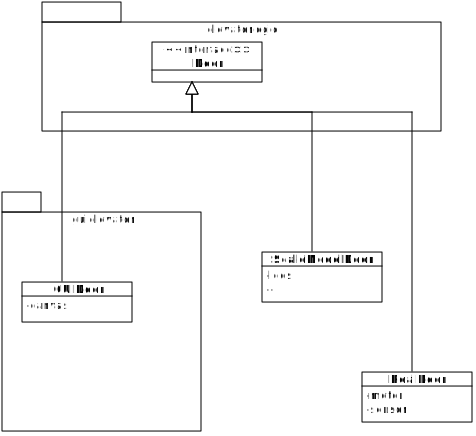
\includegraphics[width=.4\textwidth]{figures/doorsystem.pdf}
  \caption{A class diagram made with Visual Paradigm}
  \label{fig:classdiagram}
\end{wrapfigure}
If the documentation you write is a design document of some software
package, you may want to include design diagrams.
No software engineering without a UML diagrams\ldots.
You can see one generated with ``dia'', a vector drawing program that
understands the UML in figure~\ref{fig:classdiagram}
~\vpageref{fig:classdiagram}. This diagram is 'wrapped' in a \Code{wrapfigure} environment, so the text may flow around it

The diagram is not very sophisticated but shows an example of a vector
format file included via an eps$\rightarrow$ pdf conversion by
epstopdf.

Open source programs like umlet and argouml are also able to produce
vector format graphics files. And sometimes it is helpful to add a box 
that is a bit bigger then the picture you want to include.
This ensures that the so called bounding box does not cut of any lines
you want in your picture. Sometimes it is necessary to give these
tools a helping hand with inkscape, that is do a bit of tinkering to
get all details right.
\begin{figure}[htbp]
  \centering
  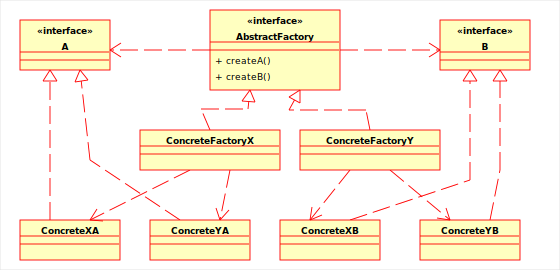
\includegraphics[width=.6\textwidth]{figures/factory}
  \caption[A class diagram by Umbrello]{A class diagram by Umbrello, saved as svg and processed
    with inkscape.}
  \label{fig:factory}
\end{figure}

% On the front cover you can find an ArgoUml diagram that shows how you could
% arrange a set of files, which would allow you to present on screen or on
% paper and in several languages from the same source files. We use this
% to prepare our freshmen syllabi and exams.

%%% Local Variables: 
%%% mode: latex
%%% TeX-master: "main"
%%% End: 

\svnidlong{$HeadURL: https://www.fontysvenlo.org/svnp/879417/latexcolloquium/trunk/latexsample/codelisting.tex $}%
{$LastChangedDate: 2014-11-16 16:03:56 +0100 (zo, 16 nov 2014) $}%
{$LastChangedRevision: 62 $}%
{$LastChangedBy: 879417 $}
\svnid{$Id: codelisting.tex 62 2014-11-16 15:03:56Z 879417 $}
\renewcommand\TheFile{codelistings.tex}

\begin{savequote}[8cm]
  \sffamily
  Use the source Luke.
  \qauthor{The most accurate documentation is in the source.}
  Addendum: Document your source well! And choose proper names.
  \qauthor{Pieter van den Hombergh}
\end{savequote}
\chapter{Listings and code documentation}
For these functions to work you need to use the \texttt{package} listings.
See mydefs.tex for the inclusion.

\lstset{%first some settings
  numbers=right, % number the lines
  numberstyle={\tiny\color{red}},frame=shadowbox,rulesepcolor=\color{gray},
  framexrightmargin=5mm
}

Note that the line numbers in the right hand border are the line
numbers in the included sources.

A good advice is to start using \define{doxygen} for your code documentation.
It can produce nicely formatted HTML and latex documents and can be
tuned in various ways with the  
help of doxywizard. The way of working is a lot like using javadoc,
but also works for C and C++ files. 
See e.g. the documentation on the zthreads package at
\url{http://zthread.sourceforge.net} or Qt at 
\url{http://doc.trolltech.com/3.3/index.html}

\section{Source code}
The most simple case: include the whole thing with a command like \\
\verb#\lstinputlisting[language=java]{code/Hi.java}#
\lstinputlisting[language=java]{code/Hi.java}

Sometimes it is useful to include just a part of a file, for instance
when you want to explain things. Like what line 11 is all about.\\
\verb#\lstinputlisting[language=java, firstline=11,lastline=11]{Hi.java}#
\lstinputlisting[language=java, firstline=11,firstnumber=11,
        lastline=11,numbers=right,basicstyle={\small\ttfamily},
        caption={use toString to let an object represent itself.}
        ]{code/Hi.java}

\section{Makefiles}
You can also include make files.
Note that makefiles have a peculiar syntax. \define{Spaces and tabs in
  Makefiles}\ are meaningful. 
That's why I made them show up in the next listing with the command\\
\lstinputlisting[firstline=65,lastline=67]{codelisting.tex}
\lstset{showspaces=true,showtabs=true}
Spaces show up as \lstinline| |, tab characters as an extended version
of the same thing (\lstinline|	|). 
As can be expected, spaces and tabs have no special meaning in
makefile comments, the lines starting with a hash (\#) sign. 
If you want to know more on makefiles try google or info:make in
konqueror on a decently installed Linux box.  

The make file for this entire document looks like this:
\lstinputlisting[language=make,showtabs=true,
     showspaces=true,basicstyle={\ttfamily\scriptsize},
     numbers=right,language=make]{Makefile}


%%% Local Variables: 
%%% mode: latex
%%% TeX-master: "main"
%%% End: 

\svnidlong{$HeadURL: https://www.fontysvenlo.org/svnp/879417/latexcolloquium/trunk/latexsample/poser.tex $}%
{$LastChangedDate: 2013-09-08 12:54:29 +0200 (Sun, 08 Sep 2013) $}%
{$LastChangedRevision: 31 $}%
{$LastChangedBy: 879417 $}
\svnid{$Id: poser.tex 31 2013-09-08 10:54:29Z 879417 $}
\renewcommand\TheFile{poser.tex}
\begin{savequote}[8cm]
  \sffamily
  Never start reading a difficult book at the wrong side.\\ 
  It makes you feel stupid.
  \qauthor{Private experience}
\end{savequote}
\chapter{So {\em you}\ know how to show off, but how do {\em I}\
  start?} 

\lstset{numberstyle={\tiny\color{red}},
  basicstyle={\small},numbers=right,
  rulesepcolor=\color{gray},
  showspaces=false,frame=shadowbox}

This document is indeed a bit of a showcase, but there is more to it.
In essence, most documents are mainly texts. 
And those plain texts take mainly typing and not much more.
The minimal, hello world style \LaTeX\ file is not much 
longer\footnote{Counting headers too!} then the C classic.
\lstinputlisting[firstline=5]{simple.tex}

And the pictures, well they are made with other packages, and as long
as those can produce a supported format, you can use them. \TeX\ and
\LaTeX\ have an own drawing language, but explaining that would blow
up this space.
There is a lot of documentation available on \TeX\ and \LaTeX\ and I
could recommend some good books on it.
But you need not run off to the nearest book shop. Lots of
documentation is on the Net, just as the \TeX\ program suite itself. 

Look for instance at \url{http://www.ntg.nl} for the Dutch \TeX\ user group
and \url{http://www.dante.de} for the German user group. They are both very 
alive and kicking.

A very good starting point nowadays is \url{http://en.wikibooks.org/wiki/LaTeX/}

\section{My own definitions}
Standard \LaTeX\ output looks a bit dull but are nicely formatted nonetheless.
If you want to make the most of your own style for your own or your
projects documentation, put your style definitions into a separate
file. That way you can keep all definitions of style and \define{macros} in one
spot. This works especially nicely in an multi part document, so
the other files (and authors) can concentrate on content.

You can \define{define} your own macros in \LaTeX. As an example a macro,
\verb#\define#, which I use
to let words stand out at the outer margin. I use it at the first use
of a word or concept in the text, to aid the reader in finding the
definition. Of course this macro could be extended to put the word
into an index. Which makes it a nice exercise.
The macro is defined as follows:\\
\lstinputlisting[frame=shadowbox,firstline=70,lastline=77]{mydefs.tex}

and is used as \verb#\define{new word}#.


%%% Local Variables: 
%%% mode: latex
%%% TeX-master: "main"
%%% End: 

\include{programmedgraphics}
\def\BackCoverMaterial{
  \setlength{\unitlength}{1mm}
  \begin{center}

  \vspace{.3\paperheight}
  \begin{picture}(160,160)
%  \begin{minipage}{\textwidth}
    \put(10,10){\includegraphics[width=120mm]{figures/TheEnd.jpg}}
%  \end{minipage}
  \end{picture}
\end{center}
\vfill
}


\end{document}
